\section{Introduction}
\label{section_ztf_intro}
Zwicky Transient Facility (\href{https://www.ztf.caltech.edu/}{ZTF}) is a time-domain survey of the northern sky
that had first light at Palomar Observatory in 2017.  It is run by CalTech.
My advisor Pavlos suggested it as a data source for this project.
The ZTF dataset has two major advantages for searching for asteroids:
\begin{itemize}
\item ZTF gives a wide and fast survey of the key, covering over 3750 square degrees an hours to a depth of 20.5 mag
\item A machine learning pipeline has been developed to classify a subset of ZTF detections that are classified as probable asteroids
\end{itemize}
The data set I analyze here consists of all ZTF detections that were classified as asteroids.
Data on each detection include:
\begin{itemize}
\item \textbf{ObjectID} an identifier of the likely ojbect associated with this detection; multiple detections often share the same ObjectID
\item \textbf{CandidateID} a unique integer identifier of each detection
\item \textbf{MJD} The time of the detection as an MJD
\item \textbf{RA} The right ascension of the detection
\item \textbf{Dec} The declination of the detection
\item \textbf{mag} The apparent magnitude of the detection
\end{itemize}
Available data also includes a number of additional fields that were not used in the analysis.

\href{https://github.com/alercebroker}{ALeRCE} (Automatic Learning for the Rapid Classification of Events) is an astronomical data broker.
ALeRCE provides a convenient API to access the ZTF asteroid data, which can be installed with \tty{pip}.
I used ALeRCE on this project to download the ZTF asteroid data set.

\section{Exploratory Data Analysis of ZTF Asteroid Data}
\label{section_ztf_eda}
Before plowing into the search for new asteroids, I conducted an exploratory data analysis (EDA) of the ZTF asteroid dataset.
This can be followed interactively in the Jupyter notebook \tty{05\_ztf\_data.ipynb}.
I took a download of the data running through 26-Feb-2020.
The first detection is on 01-Jun2018.
The dataset contains 5.69 total detections.  
The volume of detections increases very significantly beginning in July 2019; 
for practical purposes the dataset consists of 8 months of detections spanning July 2019 through February 2020.

\begin{figure}[hbt!]
\begin{center}
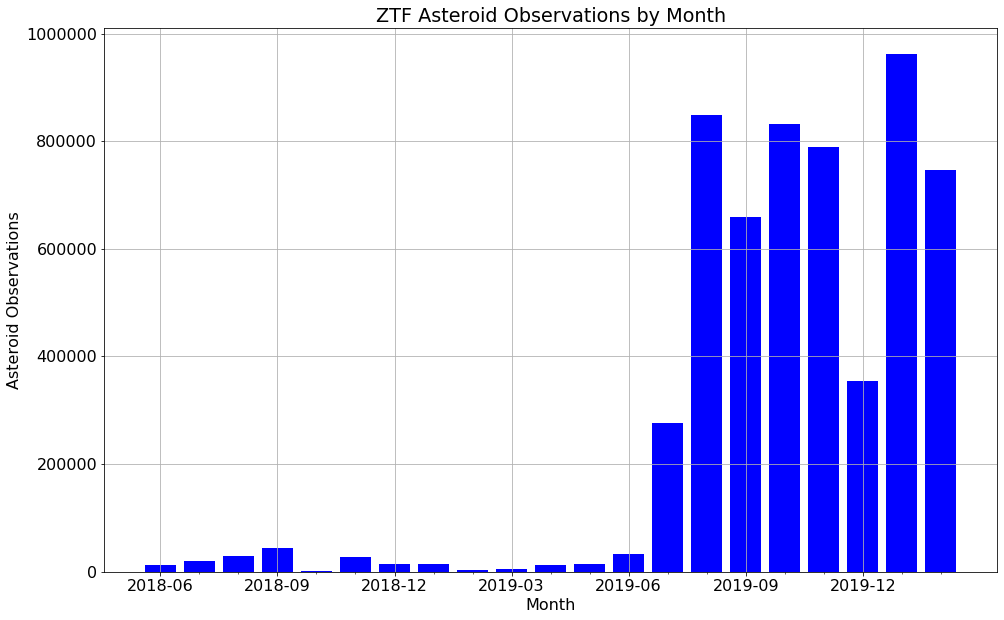
\includegraphics[width=0.8\textwidth]{../figs/ztf/ztf_ast_per_month.png}
\caption{The topographic coordinate system, courtesy of \href{https://en.wikipedia.org/wiki/Horizontal_coordinate_system}{Wikipedia}}
\end{center}
\end{figure}


\section{Finding the Nearest Asteroid to Each ZTF Observation}
\label{section_ztf_nearest_ast}

\section{Analyzing the Distribution of Distance to the Nearest Asteroid}
\label{section_nearest_ast_distribution}
\section{Setup}

% \section{Conclusion}
